% Grey swan domain overview: 4 domains x 4 event types
% Redesigned: horizontal layout, more compact, clearer connections
\documentclass[border=6pt]{standalone}
\usepackage{tikz}
\usepackage{amsmath,amssymb}
\usetikzlibrary{arrows.meta,positioning,shapes.geometric,fit,calc,backgrounds}

% Forgis brand colors — academic palette for white-background figures
% Source: color_schema.json
%
% Usage: % Forgis brand colors — academic palette for white-background figures
% Source: color_schema.json
%
% Usage: % Forgis brand colors — academic palette for white-background figures
% Source: color_schema.json
%
% Usage: \input{colors.tex} in each standalone figure .tex file.
% All figures MUST use only these colors. No inline hex.

% Brand primaries
\definecolor{ctiger}{HTML}{FF5A00}       % Primary accent (Forgis orange)
\definecolor{cfire}{HTML}{FF4D00}        % Critical
\definecolor{cflicker}{HTML}{DC4B07}     % Secondary accent
\definecolor{csteel}{HTML}{878F92}       % Muted neutral
\definecolor{cgunmetal}{HTML}{122128}    % Dark text

% Academic derived palette
\definecolor{cprimary}{HTML}{FF5A00}     % = tiger
\definecolor{cprimarylight}{HTML}{FF8C42}
\definecolor{cprimarybg}{HTML}{FFF0E6}
\definecolor{csecondary}{HTML}{2B6CB0}   % Complementary blue
\definecolor{csecondarylight}{HTML}{4A90D9}
\definecolor{csecondarybg}{HTML}{E8F0FA}
\definecolor{caccent}{HTML}{2D8A6E}      % Teal
\definecolor{caccentlight}{HTML}{5BB89A}
\definecolor{caccentbg}{HTML}{E6F5F0}
\definecolor{chighlight}{HTML}{DC4B07}   % = flicker
\definecolor{chighlightbg}{HTML}{FDEDE6}
\definecolor{ctextdark}{HTML}{122128}    % = gunmetal
\definecolor{ctextmid}{HTML}{878F92}     % = steel
\definecolor{ctextlight}{HTML}{B0B7BA}
\definecolor{cborder}{HTML}{D1D5D8}
\definecolor{cbgwarm}{HTML}{FFF8F2}
\definecolor{cbgcool}{HTML}{F4F7FA}
 in each standalone figure .tex file.
% All figures MUST use only these colors. No inline hex.

% Brand primaries
\definecolor{ctiger}{HTML}{FF5A00}       % Primary accent (Forgis orange)
\definecolor{cfire}{HTML}{FF4D00}        % Critical
\definecolor{cflicker}{HTML}{DC4B07}     % Secondary accent
\definecolor{csteel}{HTML}{878F92}       % Muted neutral
\definecolor{cgunmetal}{HTML}{122128}    % Dark text

% Academic derived palette
\definecolor{cprimary}{HTML}{FF5A00}     % = tiger
\definecolor{cprimarylight}{HTML}{FF8C42}
\definecolor{cprimarybg}{HTML}{FFF0E6}
\definecolor{csecondary}{HTML}{2B6CB0}   % Complementary blue
\definecolor{csecondarylight}{HTML}{4A90D9}
\definecolor{csecondarybg}{HTML}{E8F0FA}
\definecolor{caccent}{HTML}{2D8A6E}      % Teal
\definecolor{caccentlight}{HTML}{5BB89A}
\definecolor{caccentbg}{HTML}{E6F5F0}
\definecolor{chighlight}{HTML}{DC4B07}   % = flicker
\definecolor{chighlightbg}{HTML}{FDEDE6}
\definecolor{ctextdark}{HTML}{122128}    % = gunmetal
\definecolor{ctextmid}{HTML}{878F92}     % = steel
\definecolor{ctextlight}{HTML}{B0B7BA}
\definecolor{cborder}{HTML}{D1D5D8}
\definecolor{cbgwarm}{HTML}{FFF8F2}
\definecolor{cbgcool}{HTML}{F4F7FA}
 in each standalone figure .tex file.
% All figures MUST use only these colors. No inline hex.

% Brand primaries
\definecolor{ctiger}{HTML}{FF5A00}       % Primary accent (Forgis orange)
\definecolor{cfire}{HTML}{FF4D00}        % Critical
\definecolor{cflicker}{HTML}{DC4B07}     % Secondary accent
\definecolor{csteel}{HTML}{878F92}       % Muted neutral
\definecolor{cgunmetal}{HTML}{122128}    % Dark text

% Academic derived palette
\definecolor{cprimary}{HTML}{FF5A00}     % = tiger
\definecolor{cprimarylight}{HTML}{FF8C42}
\definecolor{cprimarybg}{HTML}{FFF0E6}
\definecolor{csecondary}{HTML}{2B6CB0}   % Complementary blue
\definecolor{csecondarylight}{HTML}{4A90D9}
\definecolor{csecondarybg}{HTML}{E8F0FA}
\definecolor{caccent}{HTML}{2D8A6E}      % Teal
\definecolor{caccentlight}{HTML}{5BB89A}
\definecolor{caccentbg}{HTML}{E6F5F0}
\definecolor{chighlight}{HTML}{DC4B07}   % = flicker
\definecolor{chighlightbg}{HTML}{FDEDE6}
\definecolor{ctextdark}{HTML}{122128}    % = gunmetal
\definecolor{ctextmid}{HTML}{878F92}     % = steel
\definecolor{ctextlight}{HTML}{B0B7BA}
\definecolor{cborder}{HTML}{D1D5D8}
\definecolor{cbgwarm}{HTML}{FFF8F2}
\definecolor{cbgcool}{HTML}{F4F7FA}


\begin{document}
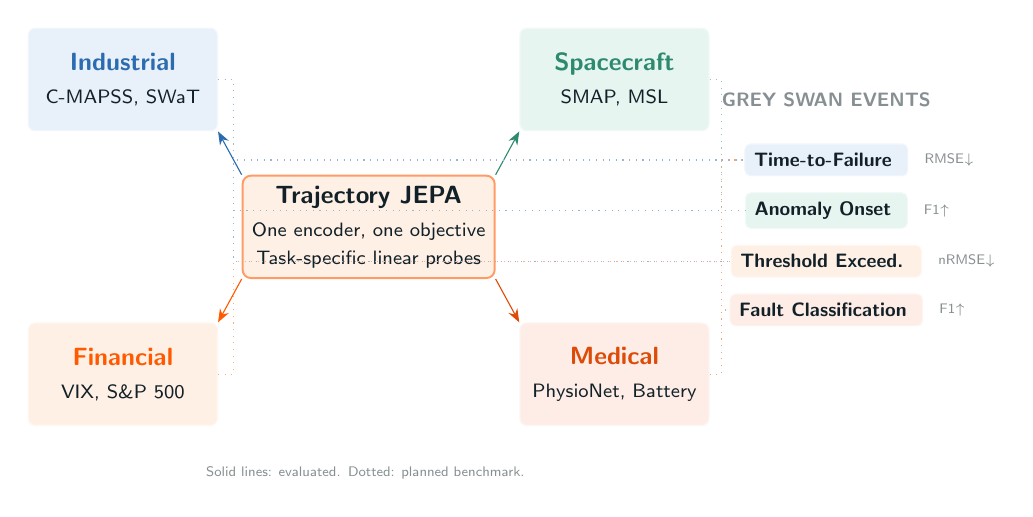
\begin{tikzpicture}[
    >=Stealth,
    font=\sffamily\small,
    dombox/.style={
        rounded corners=2.5pt,
        draw=#1!60, line width=0.5pt, fill=#1,
        minimum height=1.3cm, minimum width=2.4cm,
        align=center, text=ctextdark, inner sep=3pt,
    },
    evbox/.style={
        rounded corners=2pt,
        draw=#1!50, fill=#1,
        minimum height=0.38cm, minimum width=1.9cm,
        align=center, font=\sffamily\scriptsize, text=ctextdark,
    },
    dataarrow/.style={->,line width=0.4pt,ctextmid},
    sechead/.style={font=\sffamily\scriptsize\bfseries,text=ctextmid},
    annot/.style={font=\sffamily\scriptsize,text=ctextmid},
]

% ============================================================
% CENTER: Trajectory JEPA
% ============================================================
\node[rounded corners=3pt, draw=cprimary!60, fill=cprimarybg,
    line width=0.7pt,
    minimum height=1.3cm, minimum width=2.6cm,
    align=center, text=ctextdark] (jepa) {
    \textbf{Trajectory JEPA}\\[1pt]
    {\scriptsize One encoder, one objective}\\[-1pt]
    {\scriptsize Task-specific linear probes}
};

% ============================================================
% DOMAINS (2x2 around center, tighter spacing)
% ============================================================

\node[dombox=csecondarybg, above left=0.55cm and 0.3cm of jepa] (industrial) {
    {\small\textbf{\textcolor{csecondary}{Industrial}}}\\[1pt]
    {\scriptsize C-MAPSS, SWaT}
};

\node[dombox=caccentbg, above right=0.55cm and 0.3cm of jepa] (space) {
    {\small\textbf{\textcolor{caccent}{Spacecraft}}}\\[1pt]
    {\scriptsize SMAP, MSL}
};

\node[dombox=cprimarybg, below left=0.55cm and 0.3cm of jepa] (finance) {
    {\small\textbf{\textcolor{cprimary}{Financial}}}\\[1pt]
    {\scriptsize VIX, S\&P 500}
};

\node[dombox=chighlightbg, below right=0.55cm and 0.3cm of jepa] (medical) {
    {\small\textbf{\textcolor{chighlight}{Medical}}}\\[1pt]
    {\scriptsize PhysioNet, Battery}
};

% Arrows from JEPA to domains
\draw[dataarrow,csecondary] (jepa.north west) -- (industrial.south east);
\draw[dataarrow,caccent] (jepa.north east) -- (space.south west);
\draw[dataarrow,cprimary] (jepa.south west) -- (finance.north east);
\draw[dataarrow,chighlight] (jepa.south east) -- (medical.north west);

% ============================================================
% EVENT TYPES (right column, compact)
% ============================================================
\coordinate (evcol) at ([xshift=4.2cm]jepa.east);

\node[sechead, anchor=south] at ([yshift=1.4cm]evcol) {GREY SWAN EVENTS};

\node[evbox=csecondarybg, anchor=center] (e_rul) at ([yshift=0.85cm]evcol) {
    \textbf{Time-to-Failure}
};
\node[font=\sffamily\tiny, text=ctextmid, right=0.08cm of e_rul] {RMSE$\downarrow$};

\node[evbox=caccentbg, below=0.2cm of e_rul] (e_anom) {
    \textbf{Anomaly Onset}
};
\node[font=\sffamily\tiny, text=ctextmid, right=0.08cm of e_anom] {F1$\uparrow$};

\node[evbox=cprimarybg, below=0.2cm of e_anom] (e_tte) {
    \textbf{Threshold Exceed.}
};
\node[font=\sffamily\tiny, text=ctextmid, right=0.08cm of e_tte] {nRMSE$\downarrow$};

\node[evbox=chighlightbg, below=0.2cm of e_tte] (e_fault) {
    \textbf{Fault Classification}
};
\node[font=\sffamily\tiny, text=ctextmid, right=0.08cm of e_fault] {F1$\uparrow$};

% ============================================================
% DOTTED CONNECTIONS (domains to event types)
% ============================================================

% Industrial -> RUL, TTE, Anomaly
\draw[dotted, csecondary!50, line width=0.4pt]
    (industrial.east) -- ++(0.2,0) |- (e_rul.west);
\draw[dotted, csecondary!50, line width=0.4pt]
    (industrial.east) -- ++(0.2,0) |- (e_anom.west);
\draw[dotted, csecondary!50, line width=0.4pt]
    (industrial.east) -- ++(0.2,0) |- (e_tte.west);

% Spacecraft -> Anomaly
\draw[dotted, caccent!50, line width=0.4pt]
    (space.east) -- ++(0.15,0) |- (e_anom.west);

% Financial -> TTE
\draw[dotted, cprimary!50, line width=0.4pt]
    (finance.east) -- ++(0.2,0) |- (e_tte.west);

% Medical -> RUL, TTE, Fault
\draw[dotted, chighlight!50, line width=0.4pt]
    (medical.east) -- ++(0.15,0) |- (e_rul.west);
\draw[dotted, chighlight!50, line width=0.4pt]
    (medical.east) -- ++(0.15,0) |- (e_fault.west);

% ============================================================
% STATUS indicators (solid = evaluated, hollow = planned)
% ============================================================
\node[font=\sffamily\tiny,text=ctextmid,anchor=north,align=center]
    at ([yshift=-0.4cm]$(finance.south)!0.5!(medical.south)$) {
    Solid lines: evaluated.\enspace Dotted: planned benchmark.
};

\end{tikzpicture}
\end{document}
